% Chapter 3

\chapter{SCATS Volume Data} % Main chapter title

% For referencing the chapter elsewhere, use \ref{Chapter3}
\label{Chapter3}

% This is for the header on each page - perhaps a shortened title
\lhead{Chapter 3. \emph{SCATS Volume Data}}

%----------------------------------------------------------------------------------------
% Quotation
``There is no order in the world around us, we must adapt ourselves to the requirements of chaos
instead."

\begin{flushright}
Kurt Vonnegut, \textit{Breakfast of Champions} (1973)
\end{flushright}

% http://www.scats.com.au/files/an_introduction_to_scats_6.pdf

\section{Introduction}
SCATS (Sydney Coordinated Adaptive Traffic System) is an adaptive traffic control system.

\section{Traffic Loop Detectors}

\subsection{Handling Missing Data}


\section{Exploratory Analysis}
The following plot shows the daily, weekly, monthly and yearly average traffic volume at a site location.

\begin{figure}[htbp]
  \centering
    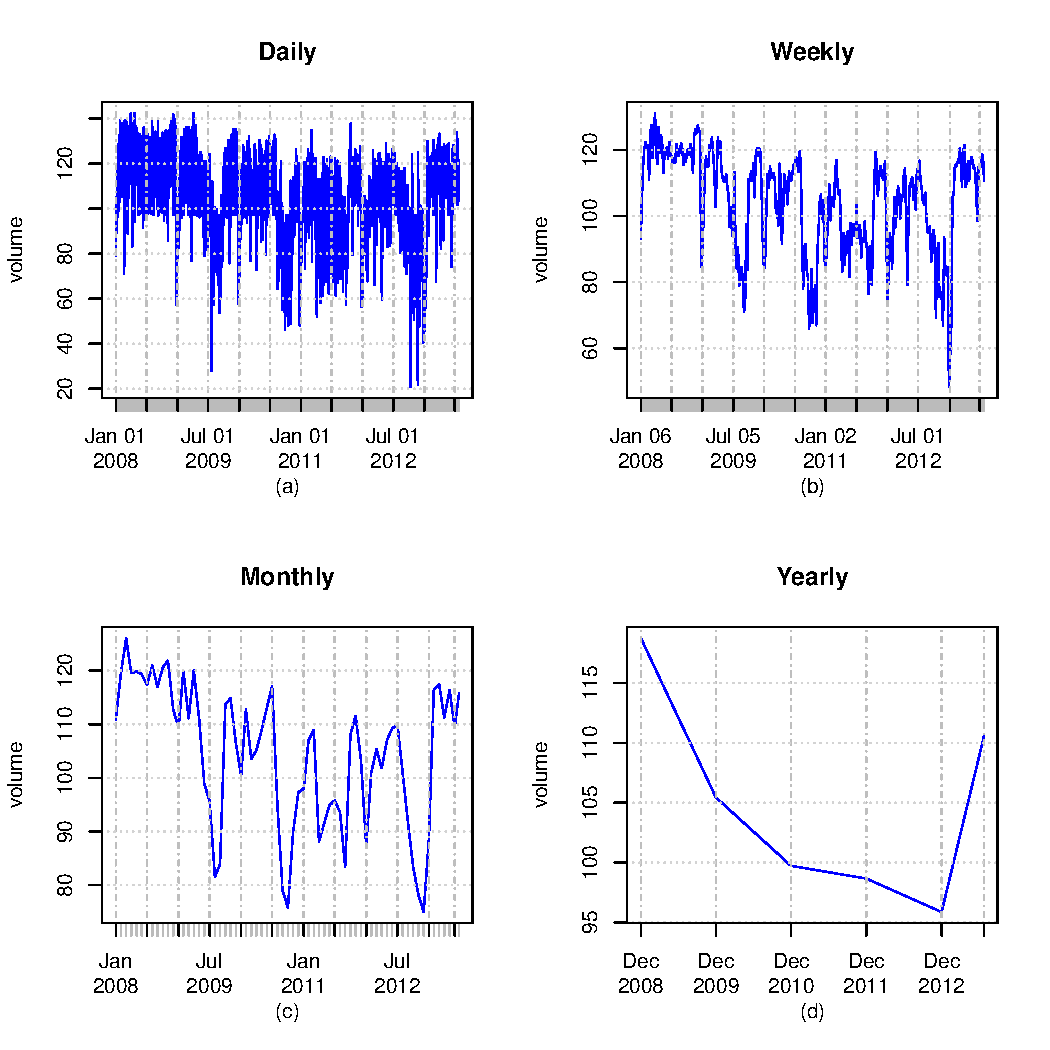
\includegraphics[width=\textwidth,height=\textheight,keepaspectratio]{Figures/averages.pdf}
    \rule{35em}{0.5pt}
  \caption[Average Traffic Volume]{(a) daily, (b) weekly, (c) monthly and (d) yearly average of traffic volume (15 mins interval) at a site location from the period 01/01/2008 to 26/07/2013}
  \label{fig:Average Traffic Volume}
\end{figure}
